\documentclass[10pt,a4paper,oneside]{article}
\usepackage[brazil]{babel}
\usepackage[utf8]{inputenc}
\usepackage{amsmath}
\usepackage{amsfonts}
\usepackage{amssymb}
\usepackage[left=3cm,right=3cm,top=2cm,bottom=2cm]{geometry}

% Floats.
\usepackage{placeins}

\usepackage{xspace}
\usepackage{graphicx}

\newcommand{\arat}{Aratibutantã\xspace}
\newcommand{\baep}{Baependinha\xspace}
\newcommand{\itam}{Itamaracanã\xspace}
\newcommand{\jaqu}{Jaquereçaba\xspace}
\newcommand{\para}{Paranapitanga\xspace}

\newcommand{\adm}{Administração\xspace}
\newcommand{\comp}{Computação e Matemática\xspace}
\newcommand{\edu}{Educacional\xspace}
\newcommand{\eng}{Engenharia e Produção\xspace}
\newcommand{\hum}{Humanidades\xspace}
\newcommand{\jur}{Jurídica e Contábil\xspace}

% Tabelas.
\usepackage{multirow}
\usepackage{booktabs}
\newcommand{\specialcell}[3][c]
{\begin{tabular}[#1]{@{}#2@{}}#3\end{tabular}}

\author{%
	Alexis A. Huf, %
	Alyson Pereira, %
	Bruno C. N. Oliveira,\\%
	Eliza Gomes, %
	Pedro H. Penna
	}

\title{Lista de Exercício I - Grupo 6}


\begin{document}

\maketitle

\paragraph{Questão 01}

A Tabela \ref{table: dados perdidos} apresenta a quantidade de dados perdidos (aqueles que não puderam ser recuperados por não estarem preenchidos) e seus respectivos percentuais em relação a cada variável analisada na base de dados em estudo. Foi observado um total de 106 dados perdidos para todas as variáveis, o que representa apenas $2.12\%$ do total. Pode-se considerar, portanto, como aceitável, uma vez que está abaixo dos $5\%$ definidos como percentual aceitável de dados perdidos.

\begin{table}[h]
\centering
\caption{Dados perdidos na base de dados.}
\label{table: dados perdidos}
\vspace{0.5em}
\begin{tabular}{c c c c c c}
	\toprule
	\textbf{Região} & \textbf{Área} & \textbf{Pagamento} & \textbf{Opinião} & \textbf{Renda} & \textbf{Idade} \\
	\midrule
	21 $(0.42\%)$   & 21 $(0.42\%)$ & 18 $(0.36\%)$      & 19 $(0.38\%)$    & 14 $(0.28\%)$  & 13 $(0.26\%)$ \\
	\bottomrule
\end{tabular}
\end{table}

%
% Dúvidas:
%   Devemos detalhar quis os erros (ex: Arábia, Araba)?
%
\paragraph{Questão 02}

A Tabela \ref{table: dados errados} resume os erros de coleta e seus respectivos percentuais na base de dados em estudo. Além de ausência de informação (conforme já mencionado na \textbf{Questão 01}), foram evidenciados erros de ortografia, digitação e formatação (ex: espaços em branco excedentes). 

As Tabelas \ref{table: erros-regiao}, \ref{table: erros-area}, \ref{table: erros-pagamento} e \ref{table: erros-opiniao} apresentam os erros observados para as variáveis qualitativas \textit{Região}, \textit{Área}, \textit{Pagamento} e \textit{Opinião}, respectivamente.
Para as variáveis quantitativas \textit{Renda} e \textit{Idade}, não foram observados erros na base de dados, isto é, valores infactíveis (ex: \textit{Renda} não positiva e \textit{Idade} inferior a 17 ou superior a 100 anos).

Para evitar que erros de ortografia e formatação sejam cometidos nas variáveis qualitativas, pode-se utilizar um formulário de múltipla escolha de modo a evitar que as informações sejam preenchidas de maneira textual. Já para as variáveis quantitativas, no caso de um formulário eletrônico, limites inferiores e superiores de valores válidos poderiam ser checado previamente à submissão da observação. Por outro lado, quanto aos dados perdidos que não foram preenchidos, é possível criar opções de modo que as pessoas possam informar explicitamente se não sabem ou, ainda, se não desejam responder. Desse modo, nenhuma informação seria ficaria perdida ou sem preenchimento. Ademais, é possível também aplicar um teste do questionário a um grupo menor de pessoas com o objetivo de testá-lo e verificar a sua adequação, para, posteriormente, aplicá-lo a um grupo maior. Assim, problemas de entendimento podem ser resolvidos nesta fase de teste, tendendo a reduzir o percentual de erros ou informações faltantes.

\begin{table}[!h]
\centering
\caption{Erros na base de dados.}
\vspace{0.5em}
\label{table: dados errados}
\begin{tabular}{c c c c c c}
	\toprule
	\textbf{Região} & \textbf{Área}  & \textbf{Pagamento} & \textbf{Opinião} & \textbf{Renda} & \textbf{Idade} \\
	\midrule
	135 $(2.71\%)$  & 114 $(2.28\%)$ & 132 $(2.64\%)$     & 123 $(2.46\%)$   & 0 $(0.00\%)$   & 0 $(0.00\%)$ \\
	\bottomrule
\end{tabular}
\end{table}

\begin{table}[!h]
\centering
\begin{minipage}[t]{0.49\textwidth}
\caption{Erros para a variável \textit{Região}.}
\vspace{0.5em}
\label{table: erros-regiao}
\begin{tabular}{l r r}
	\toprule
	\textbf{Erro} & \textbf{Absoluto}  & \textbf{Percentual} \\
	\midrule
	Arati      & 6  & $0.12\%$ \\
	Aratib     & 12 & $0.24\%$ \\
	Aratibu    & 5  & $0.10\%$ \\
	Aratibut   & 12 & $0.24\%$ \\
	Baepe      & 17 & $0.34\%$ \\
	Baepen     & 18 & $0.36\%$ \\
	Baepend    & 12 & $0.24\%$ \\
	Baependi   & 9  & $0.18\%$ \\
	Itama      & 5  & $0.10\%$ \\
	Itamar     & 6  & $0.12\%$ \\
	Itamara    & 3  & $0.06\%$ \\
	Itamarac   & 7  & $0.14\%$ \\
	Jaque      & 5  & $0.10\%$ \\
	Jaquer     & 10 & $0.20\%$ \\
	Jaquere    & 5  & $0.10\%$ \\
	Jaquereç   & 3  & $0.06\%$ \\
	\midrule
	\textbf{Total de erros}  & 135  & $2.71\%$ \\	
	\bottomrule
\end{tabular}
\end{minipage}
%
\begin{minipage}[t]{0.49\textwidth}
\caption{Erros para a variável \textit{Área}.}
\vspace{0.5em}
\label{table: erros-area}
\begin{tabular}{l r r}
	\toprule
	\textbf{Erro} & \textbf{Absoluto}  & \textbf{Percentual} \\
	\midrule
	Admin      & 3   & $0.06\%$ \\
	Admini 	   & 3   & $0.06\%$ \\
	Adminis    & 2   & $0.04\%$ \\
	Administ   & 5   & $0.10\%$ \\
	Compu      & 1   & $0.02\%$ \\
	Comput     & 2   & $0.04\%$ \\
	Computa    & 2   & $0.04\%$ \\
	Computaç   & 1   & $0.02\%$ \\
	Educa      & 2   & $0.04\%$ \\
	Educac     & 2   & $0.04\%$ \\
	Educaci    & 1   & $0.02\%$ \\
	Educacio   & 1   & $0.02\%$ \\
	Engen      & 15  & $0.30\%$ \\
	Engenh     & 9   & $0.18\%$ \\
	Engenha    & 8   & $0.16\%$ \\
	Engenhar   & 14  & $0.28\%$ \\
	Human      & 3   & $0.06\%$ \\
	Humani     & 3   & $0.06\%$ \\
	Humanid    & 4   & $0.08\%$ \\
	Humanida   & 5   & $0.10\%$ \\
	Juríd      & 3   & $0.06\%$ \\
	Jurídi     & 7   & $0.14\%$ \\
	Jurídic    & 11  & $0.22\%$ \\
	Jurídica   & 7   & $0.14\%$ \\	
	\midrule
	\textbf{Total de erros}  & 114  & $2.28\%$ \\	
	\bottomrule
\end{tabular}
\end{minipage}
\end{table}

\begin{table}[!h]
\centering
\begin{minipage}[t]{0.49\textwidth}
\caption{Erros para a variável \textit{Pagamento}.}
\vspace{0.5em}
\label{table: erros-pagamento}
\begin{tabular}{l r r}
	\toprule
	\textbf{Erro} & \textbf{Absoluto}  & \textbf{Percentual} \\
	\midrule
	Auxíl     		& 3   & $0.06\%$ \\
	Auxíli 	  		& 2   & $0.04\%$ \\
	Auxílio    	 	& 2   & $0.04\%$ \\
	Auxílio \textit{(espaço)}   	& 1   & $0.02\%$ \\
	Bolsa      	 	& 3   & $0.06\%$ \\
	Bolsas     	 	& 1   & $0.02\%$ \\
	Bolsas d   	 	& 5   & $0.10\%$ \\
	Finan      	 	& 15  & $0.30\%$ \\
	Financ     	 	& 13  & $0.26\%$ \\
	Financi    	 	& 19  & $0.38\%$ \\
	Financia   	 	& 13  & $0.26\%$ \\
	Incen      	 	& 8   & $0.16\%$ \\
	Incent     	 	& 11  & $0.22\%$ \\
	Incenti    	 	& 11  & $0.22\%$ \\
	Incentiv   	 	& 10  & $0.20\%$ \\
	Recur      	 	& 4   & $0.08\%$ \\
	Recurs     	 	& 4   & $0.08\%$ \\
	Recurso    	 	& 5   & $0.10\%$ \\
	Recursos   	 	& 2   & $0.04\%$ \\	
	\midrule
	\textbf{Total de erros}  & 132  & $2.64\%$ \\	
	\bottomrule
\end{tabular}
\end{minipage}
%
\begin{minipage}[t]{0.49\textwidth}
\caption{Erros para a variável \textit{Opinião}.}
\vspace{0.5em}
\label{table: erros-opiniao}
\begin{tabular}{l r r}
	\toprule
	\textbf{Erro} & \textbf{Absoluto}  & \textbf{Percentual} \\
	\midrule
	Indifer    & 14  & $0.28\%$ \\
	Indifere   & 16  & $0.32\%$ \\
	Insatis    & 7   & $0.14\%$ \\
	Insatisf   & 10  & $0.20\%$ \\
	Muito i    & 3   & $0.06\%$ \\
	Muito in   & 5   & $0.10\%$ \\
	Muito s    & 22  & $0.44\%$ \\
	Muito sa   & 28  & $0.56\%$ \\
	Satisfe    & 10  & $0.20\%$ \\
	Satisfei   & 8   & $0.16\%$ \\	
	\midrule
	\textbf{Total de erros}  & 123  & $2.46\%$ \\	
	\bottomrule
\end{tabular}
\end{minipage}
\end{table}


\begin{table}[!h]
\centering

\end{table}

\FloatBarrier

\paragraph{Questão 03}

A tabela de frequências para a variável \textit{Região} está indicada na Tabela \ref{table: tabela frequencias regiao}. Por análise, pode-se observar que a região predominante na base dados é \textit{\baep}, embora não represente a maioria absoluta.

\begin{table}[!h]
\centering
\caption{Frequências para a variável \textit{Região}.}
\vspace{0.5em}
\label{table: tabela frequencias regiao}
\vspace{0.5em}
\begin{tabular}{c c c c c}
	\toprule
	\textbf{\arat}    & \textbf{\baep}   & \textbf{\itam}  & \textbf{\jaqu}  & \textbf{\para} \\
	\midrule
	1185 $(23.80\%)$  & 2294 $(46.07\%)$ & 843 $(16.93\%)$ & 536 $(10.77\%)$ & 121 $(2.43\%)$ \\
	\bottomrule
\end{tabular}
\end{table}

\paragraph{Questão 04}

A tabela de frequências para a variável \textit{Área} está indicada na Tabela \ref{table: tabela frequencias area}. Por análise, pode-se observar que a \textit{Área} predominante da \texttt{TYU} modificou-se para \eng.


\begin{table}[h]
\centering
\caption{Frequências para a variável \textit{Área}.}
\vspace{0.5em}
\label{table: tabela frequencias area}
\vspace{0.5em}
\begin{tabular}{c c c c c c}
	\toprule
	\textbf{\adm}   & \textbf{\comp} & \textbf{\edu} & \textbf{\eng}    & \textbf{\hum}   & \textbf{\jur} \\
	\midrule
	592 $(11.89\%)$ & 296 $(5.94\%)$ & 338 $(6.79\%)$ & 1741 $(34.97\%)$ & 503 $(10.10\%)$ & 1509 $(30.31\%)$ \\
	\bottomrule
\end{tabular}
\end{table}


\paragraph{Questão 05}

A tabela de frequências para a variável \textit{Pagamento} está indicada na Tabela \ref{table:frequencias-pagamento}. Por análise, pode-se observar que os recursos usados para pagar as mensalidades do curso são oriundos, em sua maioria, de \textit{Financiamento Bancário} representando $43.98\%$. Já o pagamento  oriundo de \textit{Incentivos Federais} apresenta-se como o segundo mais utilizado, com  $29.06\%$.  Portanto, a maior dependência de pagamento está no \textit{Financiamento Bancário}, embora  \textit{Incentivos Federais} representem a segunda forma de pagamento mais utilizada.

\begin{table}[!h]
\centering
\caption{Frequências para a variável \textit{Pagamento}.}
\vspace{0.5em}
\label{table:frequencias-pagamento}
\begin{tabular}{c c c c c}
	\toprule
	\textbf{Aux. de Fam.}    & \textbf{Bolsas}   & \textbf{Financ. Banc.}  & \textbf{Inc. Federais} & \textbf{Rec. Próprios} \\
	\midrule
	257 $(5.16\%)$ & 328 $(6.58\%)$ & 2191 $(43.98\%)$ & 1448 $(29.06\%)$ & 758 $(15.21\%)$ \\
	\bottomrule
\end{tabular}
\end{table}

\paragraph{Questão 06}

A tabela de frequências para a variável \textit{Opinião} está indicada na Tabela \ref{table:frequencias-opiniao}. Por análise, pode-se observar que a opinião predominante na base dados é \textit{Muito satisfeito}. O grupo dos que mencionaram estarem \textit{Muito satisfeito} e \textit{Satisfeito} totaliza $55,29\%$. Podemos considerar, portanto, que a maioria dos alunos da TYU que opinaram estão satisfeitos com a EAD.

\begin{table}[!h]
\centering
\caption{Frequências para a variável \textit{Opinião}.}
\vspace{0.5em}
\label{table:frequencias-opiniao}
\begin{tabular}{c c c c c}
	\toprule
	\textbf{Indiferente}    & \textbf{Insatisfeito}   & \textbf{Muito insatisfeito}  & \textbf{Muito satisfeito} & \textbf{Satisfeito} \\
	\midrule
	1006 $(20.20\%)$ & 749 $(15.04\%)$ & 472 $(9.48\%)$ & 1719 $(34.51\%)$ & 1035 $(20.78\%)$ \\
	\bottomrule
\end{tabular}
\end{table}


\paragraph{Questão 07}
A tabela \ref{table:medidas-renda} foi construída com base nos valores de \textit{Renda} disponíveis na base de dados e apresenta as diversas medidas calculadas para análise desta variável. Vale observar que, para fins de análise, criou-se uma nova variável com base na renda multiplicando-a por 880 (valor utilizado para o salário mínimo). Pode-se observar que pelo menos três quartos dos alunos de EAD da TYU ainda mantém renda familiar inferior a $R\$2450,00$, uma vez que o quartil superior da base de dados para essa variável é de $R\$2402,40$.

Por meio da Curtose, é possível analisar também o grau de achatamento da distribuição como sendo leptocúrtica - uma curva de frequência mais aguda. Além disso, como a média e mediana são diferentes, existe uma assimetria de $9.94$, isto é, a distribuição dos dados é assimétrica à direita ou positiva. Pode-se interpretar, ademais, a dispersão de $76\%$ dos dados em relação à média, com base no Coeficiente de variação.
Com relação aos valores discrepantes, observa-se que o conjunto de dados analisados e disponíveis na base de dados contempla $296$ valores de renda acima de $4224.00$. Um histograma da variável idade é apresentado na Figura \ref{fig:histograma-renda}.

\begin{table}[!h]
\centering
\caption{Análise das medidas para a variável variável \textit{Renda}.}
\vspace{0.5em}
\label{table:medidas-renda}
\begin{tabular}{l r}
	\toprule
	\textbf{Medida}               & \textbf{Valor} \\
	\midrule
	Média                         &  $2056,05$     \\
	Moda                          &  $906,40$      \\
	Mediana                       &  $1628,00$     \\
	Variância                     &  $2449929,23$  \\
	Desvio Padrão                 &  $1565.38$     \\
	Coeficiente de Variação       &  $76\%$        \\
	Assimetria                    &  $9.94$        \\
	Curtose                       &  $253.91$      \\
	Mínimo                        &  $880.00$      \\
	Máximo                        &  $53504.00$    \\
	Quartil Inferior (Qi)         &  $1188.00$     \\
	Quartil Superior (Qs)         &  $2402.40$     \\
	Diferença Interquartil        &  $1214.40$     \\
	$Qi-1.5x(Qs-Qi)$ (Discrep. -) &  $-633.60$     \\
	$Qs+1.5x(Qs-Qi)$ (Discrep. +) &  $4224.00$     \\
	Dados Totais                  &  $5000$        \\
	Dados Válidos                 &  $4986$        \\
	Dados Perdidos                &  $14$          \\
	Dados Discrepantes            &  $296$         \\
	\bottomrule
\end{tabular}
\end{table}

\begin{figure}[!h]
	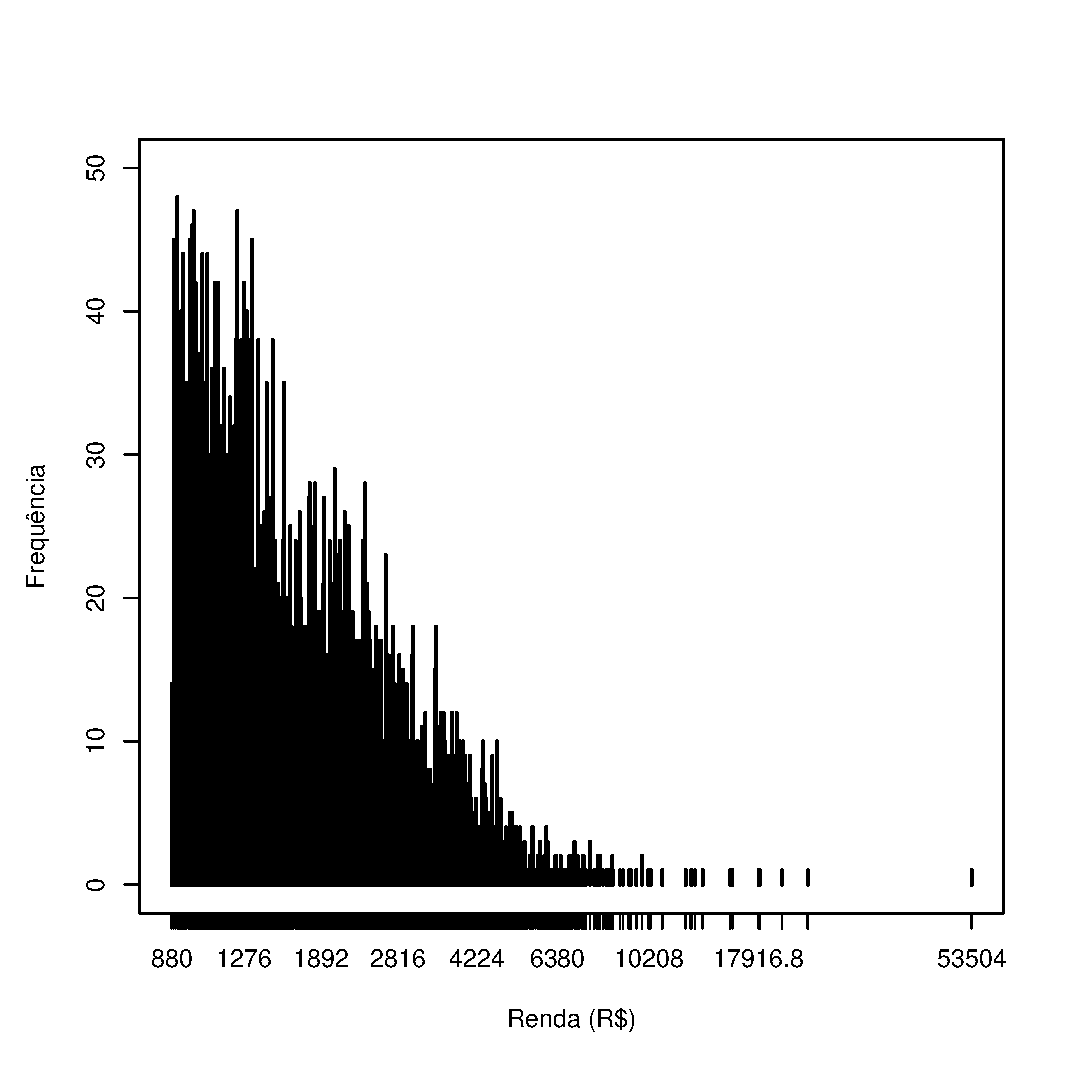
\includegraphics[width=\linewidth]{plots/histogram_renda_log.eps}
	\caption{Histograma da varável \textit{Renda}. Escala logarítimica no eixo $x$}
	\label{fig:histograma-renda}
\end{figure}

%
% {GRÁFICOS}
%

\FloatBarrier

\paragraph{Questão 08}

Algumas medidas descritivas para a variável \textit{idade} são apresentadas na Tabela \ref{table:medidas-idade}. Por análise, a maioria dos alunos de EAD na TYU possuem mais de 30 anos. Essa conclusão pode ser tomada com base mediana, que assume valor $32$ anos. Mais especificamente, a proporção de alunos com mais de 30 anos na amostra é de $61,4\%$. fazendo uma comparação com o perfil antigo, pode-se afirmar que o perfil dos alunos mudou, agora a maioria dos alunos são dois anos mais velhos, de $30$ para $32$ anos.

Fazendo uma análise mais detalhada, percebe-se que a variável em estudo segue uma distribuição com curtose leptocúrtica e assimetria positiva. Além disso, podemos observar que pelo quartil inferior e superior, que 50\%  dos alunos possuem de $29$ a $35$ anos. Vale observar, que dos 98 valores discrepantes na amostra, a maioria, 69 deles encontram-se superiores a $44$ anos. A Figura \ref{fig:histogram-idade} apresenta a distribuição de frequência da variável idade.

\begin{table}[!h]
	\centering
	\caption{Análise das medidas para a variável variável \textit{idade}.}
	\vspace{0.5em}
	\label{table:medidas-idade}
	\begin{tabular}{l r}
		\toprule
		\textbf{Medida}               & \textbf{Valor} \\
		\midrule
		Média                         &  $32.18$       \\
		Moda                          &  $32.00$       \\
		Mediana                       &  $32$          \\
		Variância                     &  $31.83$       \\
		Desvio Padrão                 &  $5.64$        \\
		Coeficiente de Variação       &  $18 \%$       \\
		Assimetria                    &  $1.205$       \\
		Curtose                       &  $6.19$        \\
		Mínimo                        &  $18$          \\
		Máximo                        &  $70$          \\
		Quartil Inferior (Qi)         &  $29$          \\
		Quartil Superior (Qs)         &  $35$          \\
		Diferença Interquartil        &  $6$           \\
		$Qi-1.5x(Qs-Qi)$ (Discrep. -) &  $20$          \\
		$Qs+1.5x(Qs-Qi)$ (Discrep. +) &  $44$          \\
		Dados Totais                  &  $5000$        \\
		Dados Válidos                 &  $4987$        \\
		Dados Perdidos                &  $13$          \\
		Dados Discrepantes            &  $98$          \\ %69 são >
		\bottomrule
	\end{tabular}
\end{table}

\begin{figure}[!h]
	\centering
	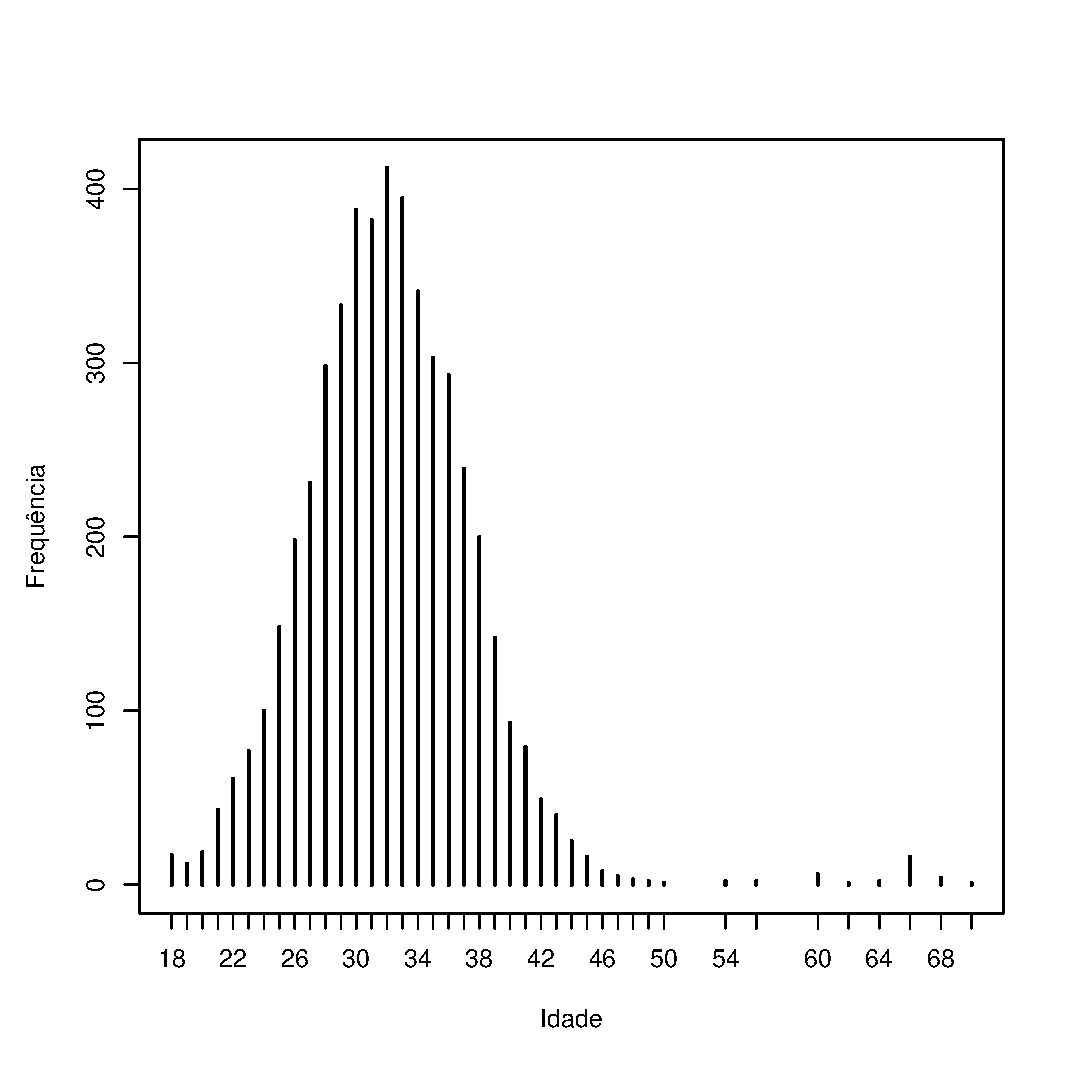
\includegraphics[width=\linewidth]{plots/histogram_idade_log.eps}
	\caption{Histograma da variável idade. }
	\label{fig:histogram-idade}
\end{figure}

\FloatBarrier

\paragraph{Questão 09}

A Tabela \ref{table:satisfacao-regiao} apresenta a satisfação por região na avaliação antiga e atual. Por análise conclui-se que o perfil atual difere-se do antigo. Para as regiões \jaqu e \para, observou-se que a avaliação dos alunos piorou. Já para as demais regiões, percebeu-se uma melhoria na avaliação. Vale ressaltar que na avaliação atual, $55,29\%$ dos alunos estão satisfeitos. No entanto, os \textit{campi} que concentram as maiores taxas de insatisfação (\arat e \para) contém apenas $26,12\%$ dos alunos. Adicionalmente \baep, que concentra avaliações dos alunos em satisfeitos e muito satisfeitos, concentra $45,88\%$ dos alunos.

\begin{table}
	\centering
	\caption{Satisfação por região.}
	\vspace{0.5em}
	\label{table:satisfacao-regiao}
	\begin{tabular}{l l l}
		\toprule
		Região & Avaliação Antiga & Avaliação Atual                                           \\
		\midrule
		\arat  & Muito Insatisfeito & Indiferente ($38,48\%$) e Insatisfeito ($32,15\%$)      \\
		\baep  & Muito Insatisfeito & Satisfeito ($33,96\%$) e Muito Satisfeito ($38,19\%$)   \\
		\itam  & Satisfeito         & Muito Satisfeito ($93,94\%$)                            \\
		\jaqu  & Indiferentes       & Insatisfeito ($33,93\%$) e Muito Satisfeito ($44,03\%$) \\
		\para  & Diversas           & Muito Insatisfeito ($91,74\%$)                          \\
		\bottomrule
	\end{tabular}
\end{table}

\paragraph{Questão 10}


\begin{table}
\centering
\begin{tabular}{l r r r r r}
	\toprule
	Curso                   & Indiferente & Insatisfeito & \specialcell{c}{Muito\\Insatisfeito} &  \specialcell{c}{Muito\\Satisfeito} & Satisfeito \\
	\midrule
	Administração           & $11.04\%$   & $3.57\%$     & $0.34\%$           & $56.37\%$        & $28.69\%$  \\
	Computação e Matemática & $18.98\%$   & $5.08\%$     & $0.68\%$           & $44.41\%$        & $30.85\%$  \\
	Educacional             & $1.78\%$    & $0.59\%$     & $0.00\%$           & $89.91\%$        & $7.72\%$   \\
	Engenharia e Produção   & $27.8\%$    & $14.26\%$    & $3.93\%$           & $27.25\%$        & $26.67\%$  \\
	Humanidades             & $6.77\%$    & $1.59\%$     & $0.00\%$           & $74.90\%$        & $16.73\%$  \\
	Jurídica e Contábil     & $23.6\%5$   & $30.17\%$    & $26.45\%$          & $6.45\%$         & $13.29\%$  \\
	\bottomrule
\end{tabular}
\end{table}

De um modo geral, o investimento resultou em uma melhora da avaliação dos cursos \edu, \hum e \eng, e estabilidade na avaliação para curso de \comp. Portanto, o investimento foi eficaz.

Na avaliação antiga  os cursos de Educacional e de Humanidades estavam muito insatisfeitos, atualmente $89.91\%$ dos alunos da área Educacional estão muito satisfeitos e $74.9\%$ dos alunos de Humanidades estão muitos satisfeitos.

Na avaliação antiga os cursos de Computação e Matemática e de Administração elogiavam seus cursos, atualmente essa característica se mantêm. Para o curso de Computação e Matemática e o Curso de Administração, $75,26\%$ e $85.09\%$ dos alunos reportaram estarem satisfeitos ou muito satisfeitos, respectivamente.

Na avaliação antiga os demais cursos (Engenharia e Produção e Jurídica e Contábil) eram indiferentes quanto ao grau de satisfação. Atualmente essa característica foi alterada. No curso de Engenharia a quantidade de pessoas satisfeitas e muito satisfeitas corresponde a um total de $53.82\%$, enquanto o percentual de alunos indiferentes é de $27.89\%$. Já para o curso de Jurídica e Contábil, o percentual de alunos insatisfeitos é alta, correspondendo a um total de $56.62\%$ do total de alunos. Do restante, $23.65\%$ se manifestaram indiferentes e apenas $19.74\%$ se consideram satisfeitos ou muito satisfeitos.

\paragraph{Questão 11}

As fontes de pagamento para cada uma das regiões são apresentadas em termos absolutos e percentuais na Tabela \ref{tabela: fontes de pagamento absoluto} e na Tabela \ref{tabela: fontes de pagamento percentual}, respectivamente. Adicionalmente, dados da Tabela \ref{tabela: fontes de pagamento percentual} são apresentados em formato gráfico na Figura \ref{figure: fonte de pagemento}.

Tanto para a região \baep quanto as demais, pode-se constar uma mudança na composição da fonte de recursos para pagamentos em relação à pesquisa anterior. Para a região \baep, a nova principal fonte de recursos é oriunda de \textit{Financiamento Bancário} ($53,01\%$). Em contraste com a pesquisa anterior, \textit{Incentivos Federais} agora compõem $15,08\%$ dos recursos. Para as regiões \itam, \jaqu e \para, um observa-se a predominância de uma única fonte de pagamento, sendo para primeira região \textit{Financiamento Bancário}, e para as demais \textit{Incentivos Federais}. Por fim, para a região \arat, observa-se uma maior participação, mas não majoritária, de \textit{Incentivos Federais} na fonte de recursos ($47,51\%$). Cabe ressaltar que \arat e \baep apresentam composições similares para os recursos de pagamentos, mas com fontes predominantes distintas.

\begin{table}
\small
\caption{Fontes de pagamento para regiões em valores absolutos.}
\label{tabela: fontes de pagamento absoluto}
\vspace{0.5em}
\begin{tabular}{l r r r r r}
	\toprule
	\textbf{Fonte Pagamento}     & \textbf{\arat}     & \textbf{\baep}   & \textbf{\itam}  & \textbf{\jaqu} & \textbf{\para}  \\
	\midrule
	Auxílio de Familiares  & $97$       & $131$  & $10$   & $17$  & $1$    \\
	Bolsas de Estudo       & $116$      & $159$  & $7$    & $43$  & $2$    \\
	Financiamento Bancário & $180$      & $1216$ & $767$  & $20$  & $0$    \\
	Incentivos Federais    & $563$      & $346$  & $3$    & $411$ & $116$  \\
	Recursos Próprios      & $226$      & $433$  & $53$   & $43$  & $1$    \\
	\bottomrule
\end{tabular}
\end{table}

\begin{table}
\small
\caption{Fontes de pagamento para regiões em valores percentuais.}
\label{tabela: fontes de pagamento percentual}
\vspace{0.5em}
\begin{tabular}{l r r r r r}
	\toprule
	\textbf{Fonte Pagamento} & \textbf{\arat}     & \textbf{\baep}   & \textbf{\itam}   & \textbf{\jaqu} & \textbf{\para}  \\
	\midrule
	Auxílio de Familiares       & $8,19\%$           & $5,71\%$         & $1,19\%$         & $3,17\%$       & $0,83\%$  \\
	Bolsas de Estudo            & $9,79\%$           & $6,93\%$         & $0,83\%$         & $8,02\%$       & $1,65\%$  \\
	Financiamento Bancário      & $15,19\%$          & $53,01\%$        & $90,98\%$        & $3,73\%$       & $0,0\%$   \\
	Incentivos Federais         & $47,51\%$          & $15,08\%$        & $0,36\%$         & $76,68\%$      & $95,87\%$ \\
	Recursos Próprios           & $19,07\%$          & $18,88\%$        & $6,29\%$         & $8,02\%$       & $0,83\%$  \\
	\bottomrule
\end{tabular}
\end{table}

\begin{figure}
\centering
	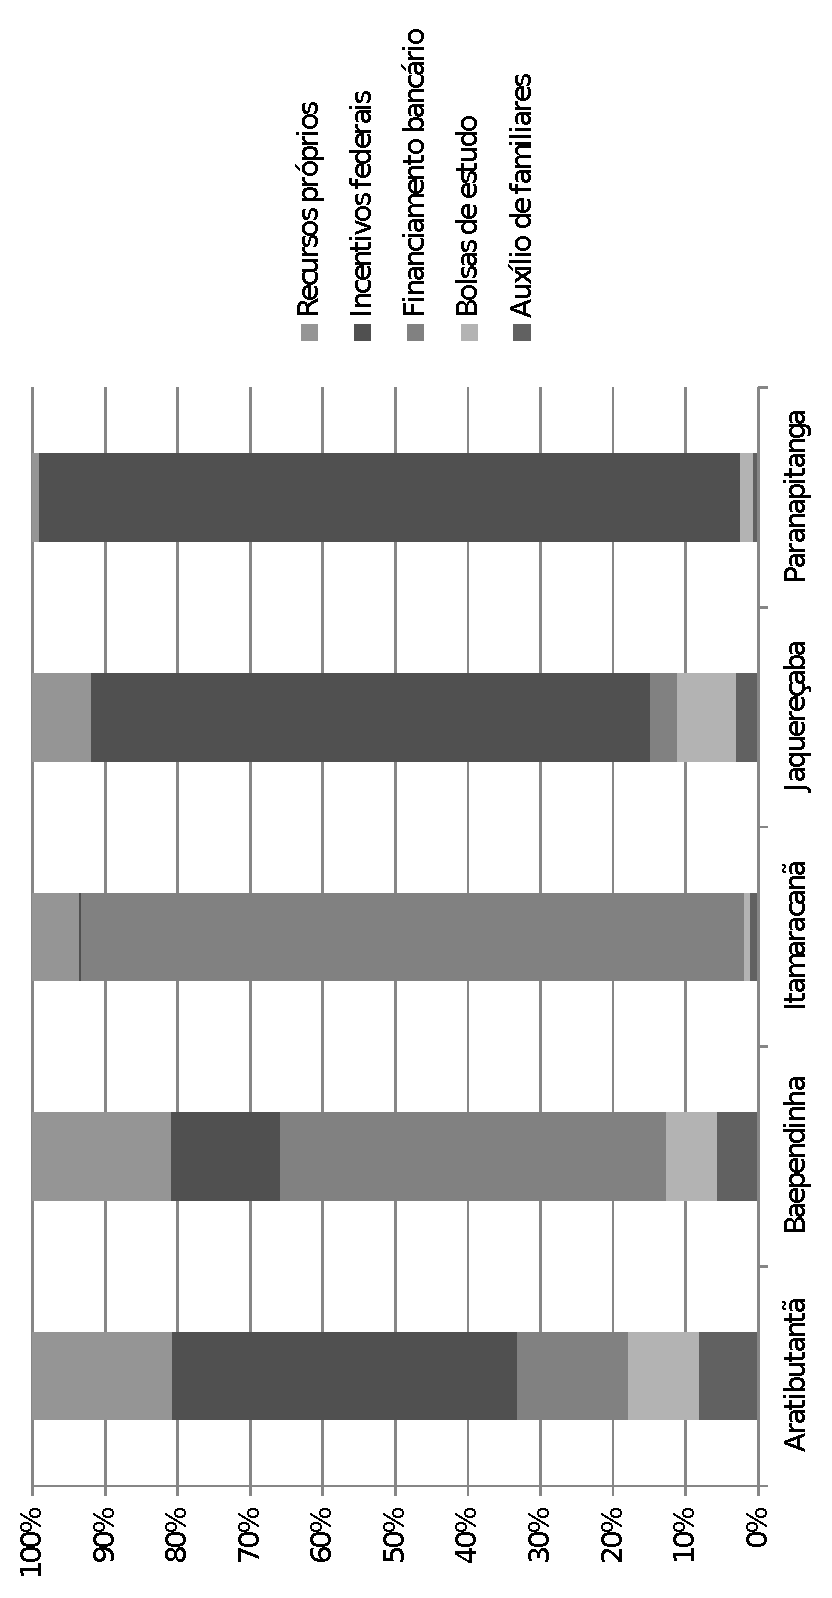
\includegraphics[width=0.80\linewidth]{plots/q11}
	\caption{Fontes de pagamento por região.}
	\label{figure: fonte de pagemento}
\end{figure}

\FloatBarrier
\paragraph{Questão 12}

A avaliação dos alunos de acordo com a fonte dos recursos para pagamento é mostrada, em valores absolutos na Tabela \ref{table: avaliacao por fonte de pagamento}, e em valores percentuais, com relação ao número de alunos utilizando determinada fonte, na Tabela \ref{table: avaliacao por fonte de pagamento-percent}. A Figura \ref{figure: avaliacao por fonte de pagamento} mostra os mesmos dados da Tabela \ref{table: avaliacao por fonte de pagamento-percent} na forma de um gráfico de barras empilhado. As fontes de recursos podem ser divididas em duas categorias, uma onde o aluno efetivamente paga pelas mensalidades, e outra onde o o aluno não paga. O primeiro grupo é composto por \textit{Financiamento Bancário} e \textit{Recursos próprios}, enquanto o segundo é composto por \textit{Auxílio de Familiares}, \textit{Bolsas de Estudo} e \textit{Incentivos Federais}. Os resultados dessa agregação são exibidos na Tabela \ref{table:pagantes-absoluto} em valores absolutos e percentuais.

A suspeita da direção da TYU de que os alunos que recebem auxílio financeiro de alguém não são tão críticos da EAD quanto os demais, não se confirma. O grupo de alunos pagantes possui avaliações significativamente melhores de seus cursos, com $83.75\%$ dos alunos avaliando os cursos como \textit{Satisfatório} ou \textit{Muito Satisfatório}. Já entre os alunos não-pagantes, apenas $18.29\%$ se declaram \textit{Satisfeitos} ou \textit{Muito Satisfeitos}, enquanto $53.26\%$ dos alunos se declararam \textit{Muito Insatisfeitos} ou \textit{Insatisfeitos} e $36.96\%$ se declaram indiferentes. Os alunos não-pagantes são na verdade o grupo de alunos mais críticos ao EAD da TYU.

\begin{figure}
	\centering
	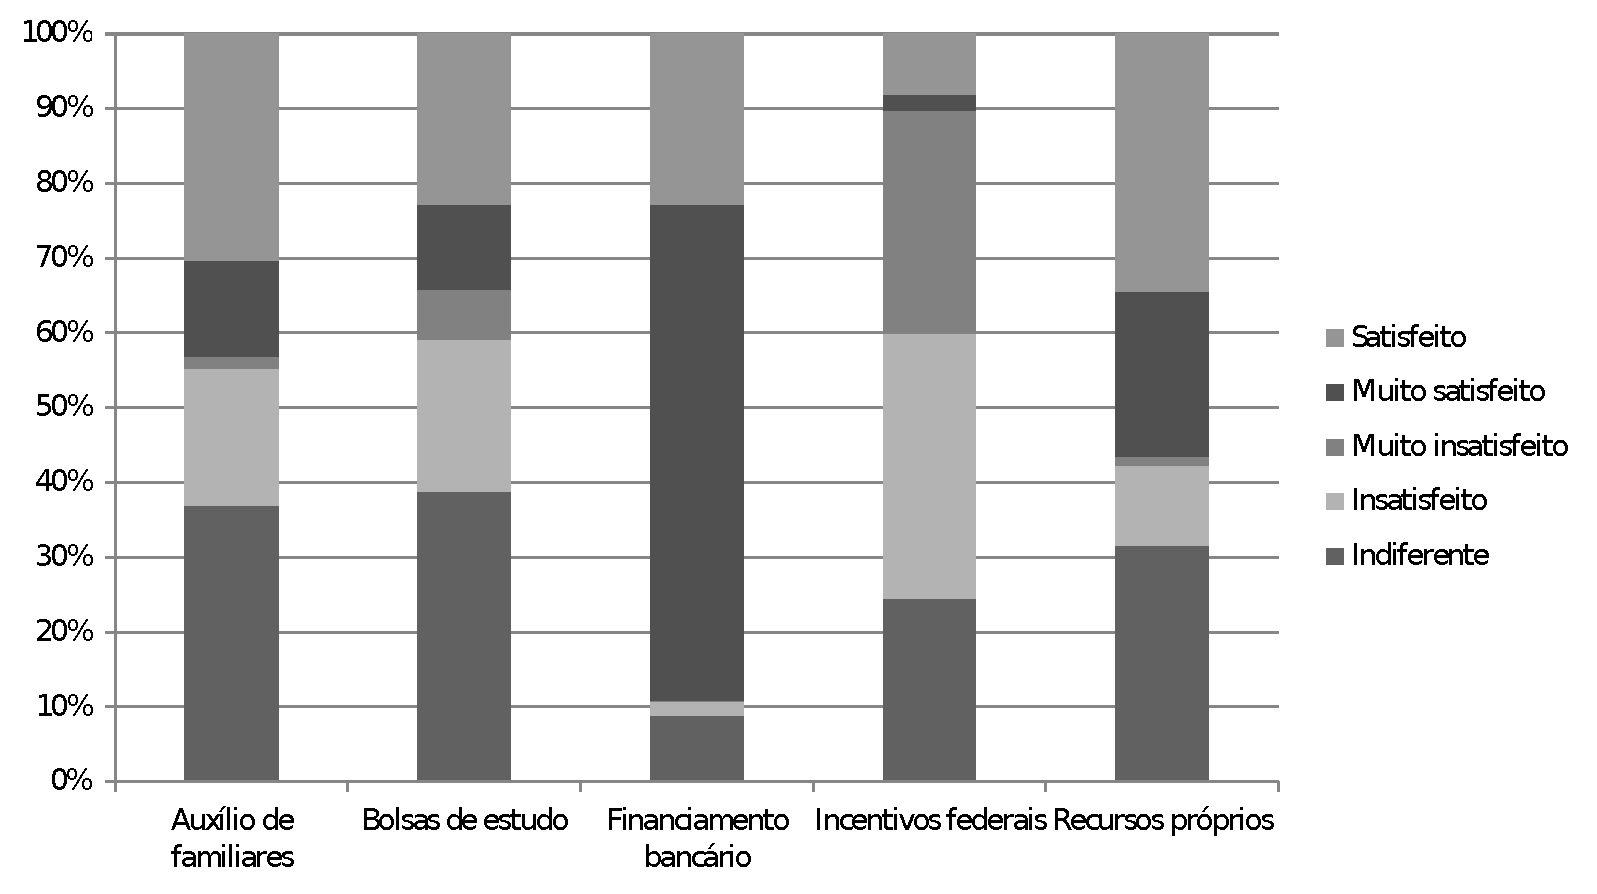
\includegraphics[width=0.80\linewidth]{plots/q12}
	\caption{Avaliação dos alunos pela fonte de pagamento}
	\label{figure: avaliacao por fonte de pagamento}
\end{figure}

\begin{table}
	\small
	\caption{Avaliação dos alunos pela fonte de pagamento.}
	\label{table: avaliacao por fonte de pagamento}
	\vspace{0.5em}
	\begin{tabular}{l r r r r r}
		\toprule
		\textbf{Fonte Pagamento}     & \textbf{Muito Insatisfeito}     & \textbf{Insatisfeito}   & \textbf{Indiferente}  & \textbf{Satisfeito} & \textbf{Muito Satisfeito}  \\
		\midrule
		Auxílio de Familiares  & $4$      & $47$   & $95$   & $78$   & $33$   \\
		Bolsas de Estudo       & $22$     & $67$   & $127$  & $75$   & $37$   \\
		Financiamento Bancário & $3$      & $42$   & $192$  & $497$  & $1448$ \\
		Incentivos Federais    & $431$    & $509$  & $354$  & $118$  & $30$   \\
		Recursos Próprios      & $9$      & $81$   & $238$  & $260$  & $166$  \\
		\bottomrule
	\end{tabular}
\end{table}


\begin{table}
	\small
	\caption{Avaliação dos alunos pela fonte de pagamento. Valores percentuais\protect\footnotemark.}
	\label{table: avaliacao por fonte de pagamento-percent}
	\vspace{0.5em}
	\begin{tabular}{l r r r r r}
		\toprule
		\textbf{Fonte Pagamento}     & \textbf{Muito Insatisfeito}     & \textbf{Insatisfeito}   & \textbf{Indiferente}  & \textbf{Satisfeito} & \textbf{Muito Satisfeito}  \\
		\midrule
		Auxílio de Familiares  & $1.56\%$    & $18.29\%$    & $36.96\%$   & $30.35\%$  & $12.84\%$  \\
		Bolsas de Estudo       & $6.71\%$    & $20.43\%$    & $38.72\%$   & $22.87\%$  & $11.28\%$  \\
		Financiamento Bancário & $0.14\%$    & $1.92\%$     & $8.76\%$    & $22.68\%$  & $66.09\%$  \\
		Incentivos Federais    & $29.77\%$   & $35.15\%$    & $24.45\%$   & $8.15\%$   & $2.07\%$   \\
		Recursos Próprios      & $1.19\%$    & $10.69\%$    & $31.40\%$   & $21.90\%$  & $34.30\%$  \\
		\bottomrule
	\end{tabular}
	
\end{table}

\footnotetext{Valores perdidos não são apresentados, mas são contabilizados no cálculo da porcentagem.}

%           Mins ins   indif sats  Msats   Total
% Paga      12   123   430   757   1614    2936
% Não paga  457  623   576   271   100     2027

\begin{table}
	\small
	\caption{Números de avaliações para alunos nas categorias agrupadas de pagantes e não-pagantes}
	\label{table:pagantes-absoluto}
	\begin{tabular}{l c c c c c}
		\toprule
		\textbf{Categoria}     & \textbf{Muito Insatisfeito}     & \textbf{Insatisfeito}   & \textbf{Indiferente}  & \textbf{Satisfeito} & \textbf{Muito Satisfeito}  \\
		\midrule
		Pagante & 12 ($0.40\%$)  & 123 ($4.18\%$)  & 430 ($36.96\%$)   & 757 ($25.78\%$)  & 1614 ($57.97\%$)  \\
		Não-pagante  & 457 ($22.54\%$) & 623 ($30.73\%$) & 576 ($36.96\%$)   & 271 ($13.36\%$)  & 100 ($4.93\%$)  \\
		\bottomrule
	\end{tabular}
\end{table}

%           Mins  ins   indif  sats   Msats   Total
% Paga      0.40  4.18  14.64  25.78  54.97    2936
% Não paga  22.54 30.73 28.41  13.36  4.93     2027

\FloatBarrier

\paragraph{Questão 13}

%Considerou-se pobres os alunos que possuem uma renda de até 1.35 salários minimos, alunos intermediarios os que recebem entre 1.35 e 2.73 salarios minimos e como abastados os que recebem acima de 2.73 salarios minimos. Isso foi baseado no quartil inferior e superior dos dados.
%#Não se observa relação entre o perfil economico dos alunos e seu grau de satisfação com a TYU, visto que a distribuição é similar para qualquer classe.

Para dividir a amostra em conjuntos de alunos pobres, com renda intermediária, e abastados foram utilizados os quartis inferior e superior. O quartil inferior foi calculado em $1.35$ salários mínimos, o que foi usado para definir todos os alunos com renda menor ou igual a $1.35$ salários como pobres. Similarmente, todos os alunos com renda superior ao quartil superior ($2.73$ salários mínimos) foram considerados como abastados. Os alunos com renda maior que $1.35$ e menor que $2.73$ foram considerados como de renda intermediária.

Usando essa divisão de classes, a contagem e percentuais associados exibidos na Tabela \ref{fig:satisfaceo-renda} foram obtidos. A Figura \ref{fig:satisfacao-renda} mostra um gráfico empilhado com a distribuição das avaliações de acordo com a classe de renda. Observando as proporções na \ref{table:satisfaca-renda}, não podem ser observadas diferenças significativas entre as avaliações das classes.

% TODO afirmação subjetiva sem embasamento.

\begin{table}[!h]
	\caption{Satisfação alunos de acordo com classes de renda.}
	\label{table:satisfaca-renda}
	\begin{tabular}{l r r r r r}
		\toprule
		\textbf{Classe} & \textbf{Muito Insatisfeito}     & \textbf{Insatisfeito}   & \textbf{Indiferente}  & \textbf{Satisfeito} & \textbf{Muito Satisfeito}  \\
		\midrule
 		 Pobres         & 256 ($20.4\%$) & 178 ($14.2\%$) & 130 ($10.4\%$) & 428 ($34.2\%$) & 260 ($20.8\%$) \\
		 Intermediário  & 505 ($20.4\%$) & 369 ($14.9\%$) & 234 ($9.4\%$)  & 874 ($35.2\%$) & 499 ($20.1\%$) \\
 		 Abastados      & 245 ($19.6\%$) & 202 ($16.2\%$) & 108 ($8.7\%$)  & 417 ($33.4\%$) & 276 ($22.1\%$) \\
		\bottomrule
	\end{tabular}
\end{table}

\begin{figure}[!h]
	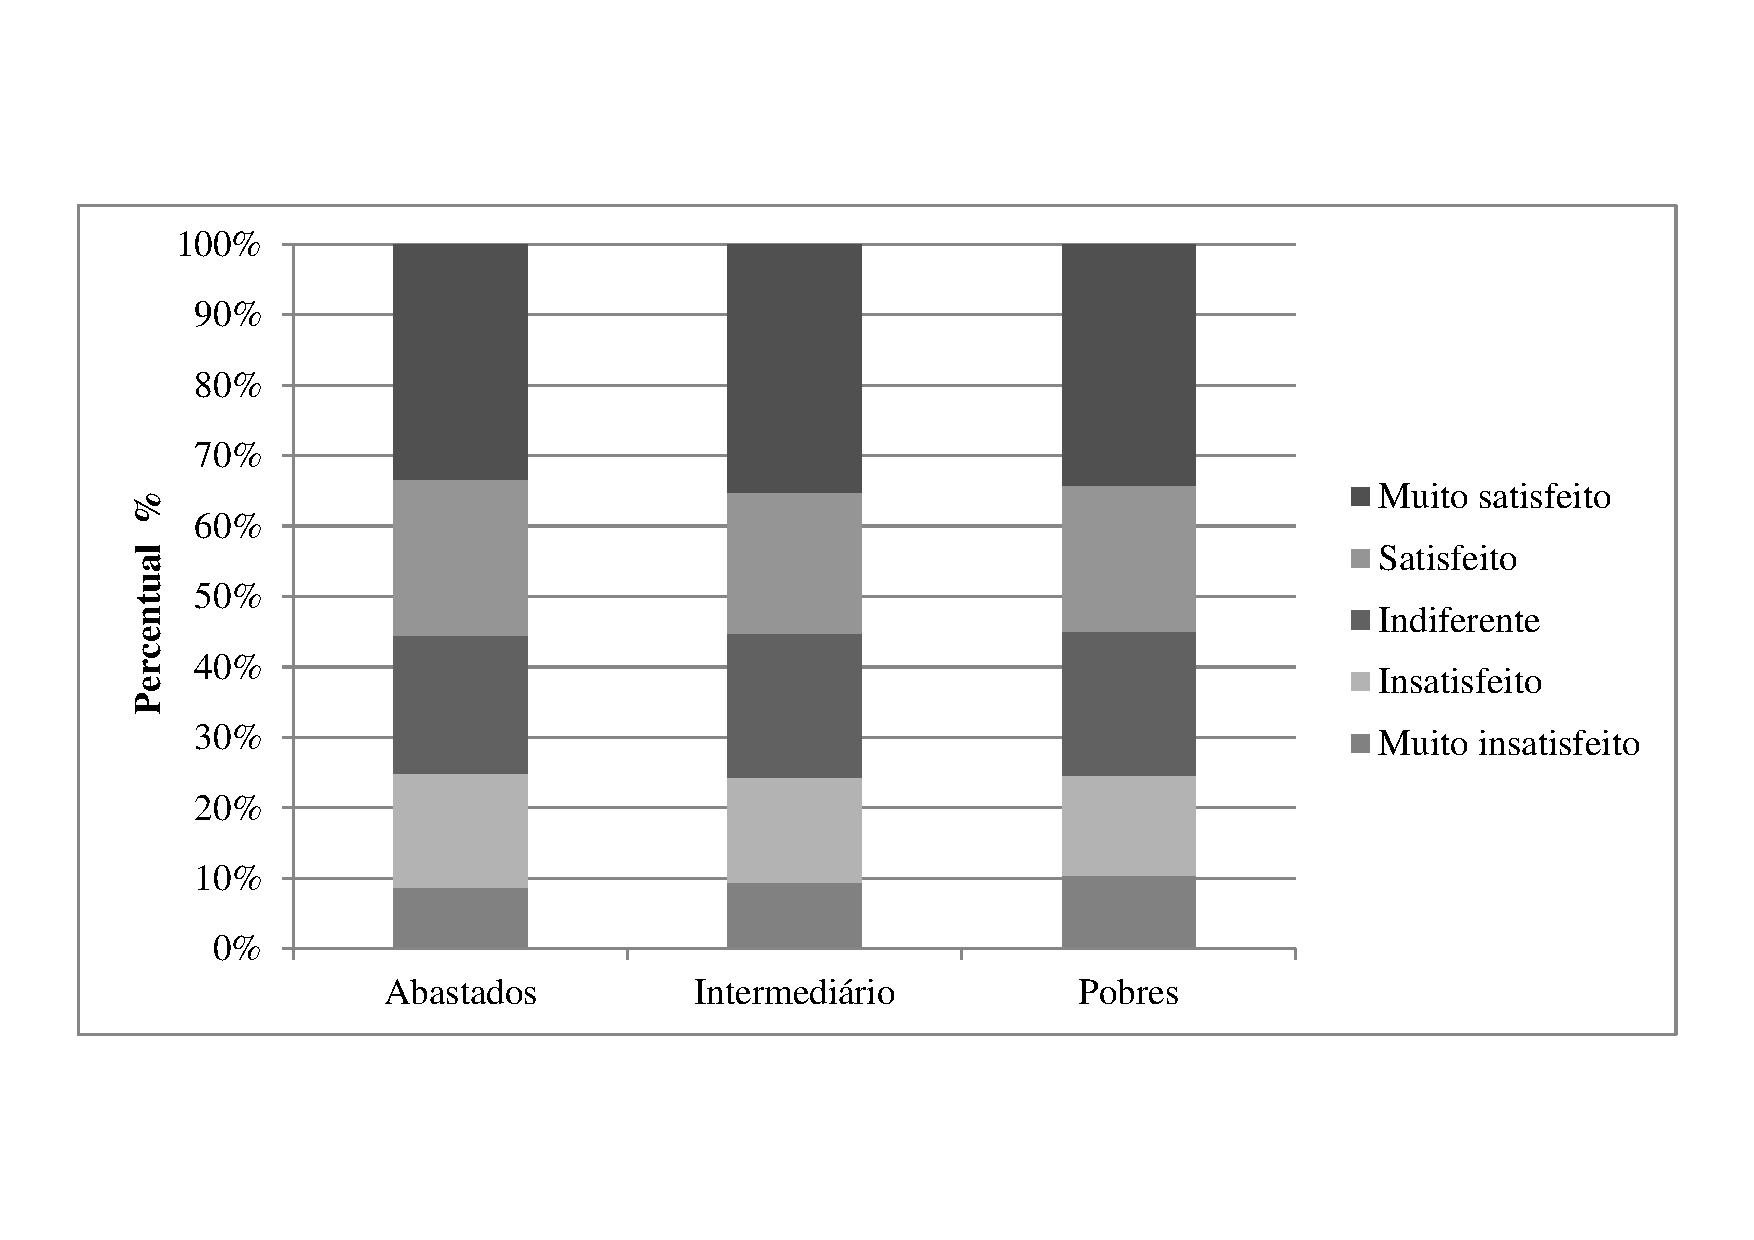
\includegraphics[width=\linewidth]{plots/q13.pdf}
	\caption{Satisfação dos alunos de acordo com classes de renda.}
	\label{fig:satisfacao-renda}
\end{figure}


\end{document}